\chapter{Segurança com \textit{firewall}}\label{chp:firewall}
%%% https://www.geeksforgeeks.org/basic-firewall-configuration-in-cisco-packet-tracer/
%%% https://www.techiesdiary.com/how-to/create-vpn-using-cisco-packet-tracer-5-3
%%% https://www.youtube.com/watch?v=gOmrso1El-o

Neste capítulo vamos abordar a utilização de um \textit{firewall} como uma ferramenta para aumentar a segurança em um servidor. Um \textit{firewall} é um mecanismo (\textit{harware} ou \textit{software}) que libera ou nega um tráfego de dados em um conjunto de endereços IP e portas lógicas. A negação ou liberação de um determinado tráfego de dados por \textit{firewall} é estabelecido através de regras de segurança ou políticas de segurança. Assim, limita-se o tráfego a serviços bem determinados e evita que conexões desconhecidas sobrecarreguem o servidor.

Para o laboratório proposto neste capítulo, vamos tomar como base a infraestrutura descrita na \Cref{fig:firewallBase} a seguir. O \textit{firewall} será configurado no servidor. Além do servidor, a rede é composta por duas redes locais, cada uma delas com dois PCs interligados por um \textit{switch} (Modelo 2960); e um roteador, que vai interligar as duas redes ao servidor.

\begin{figure}[!hbt]
    \centering
    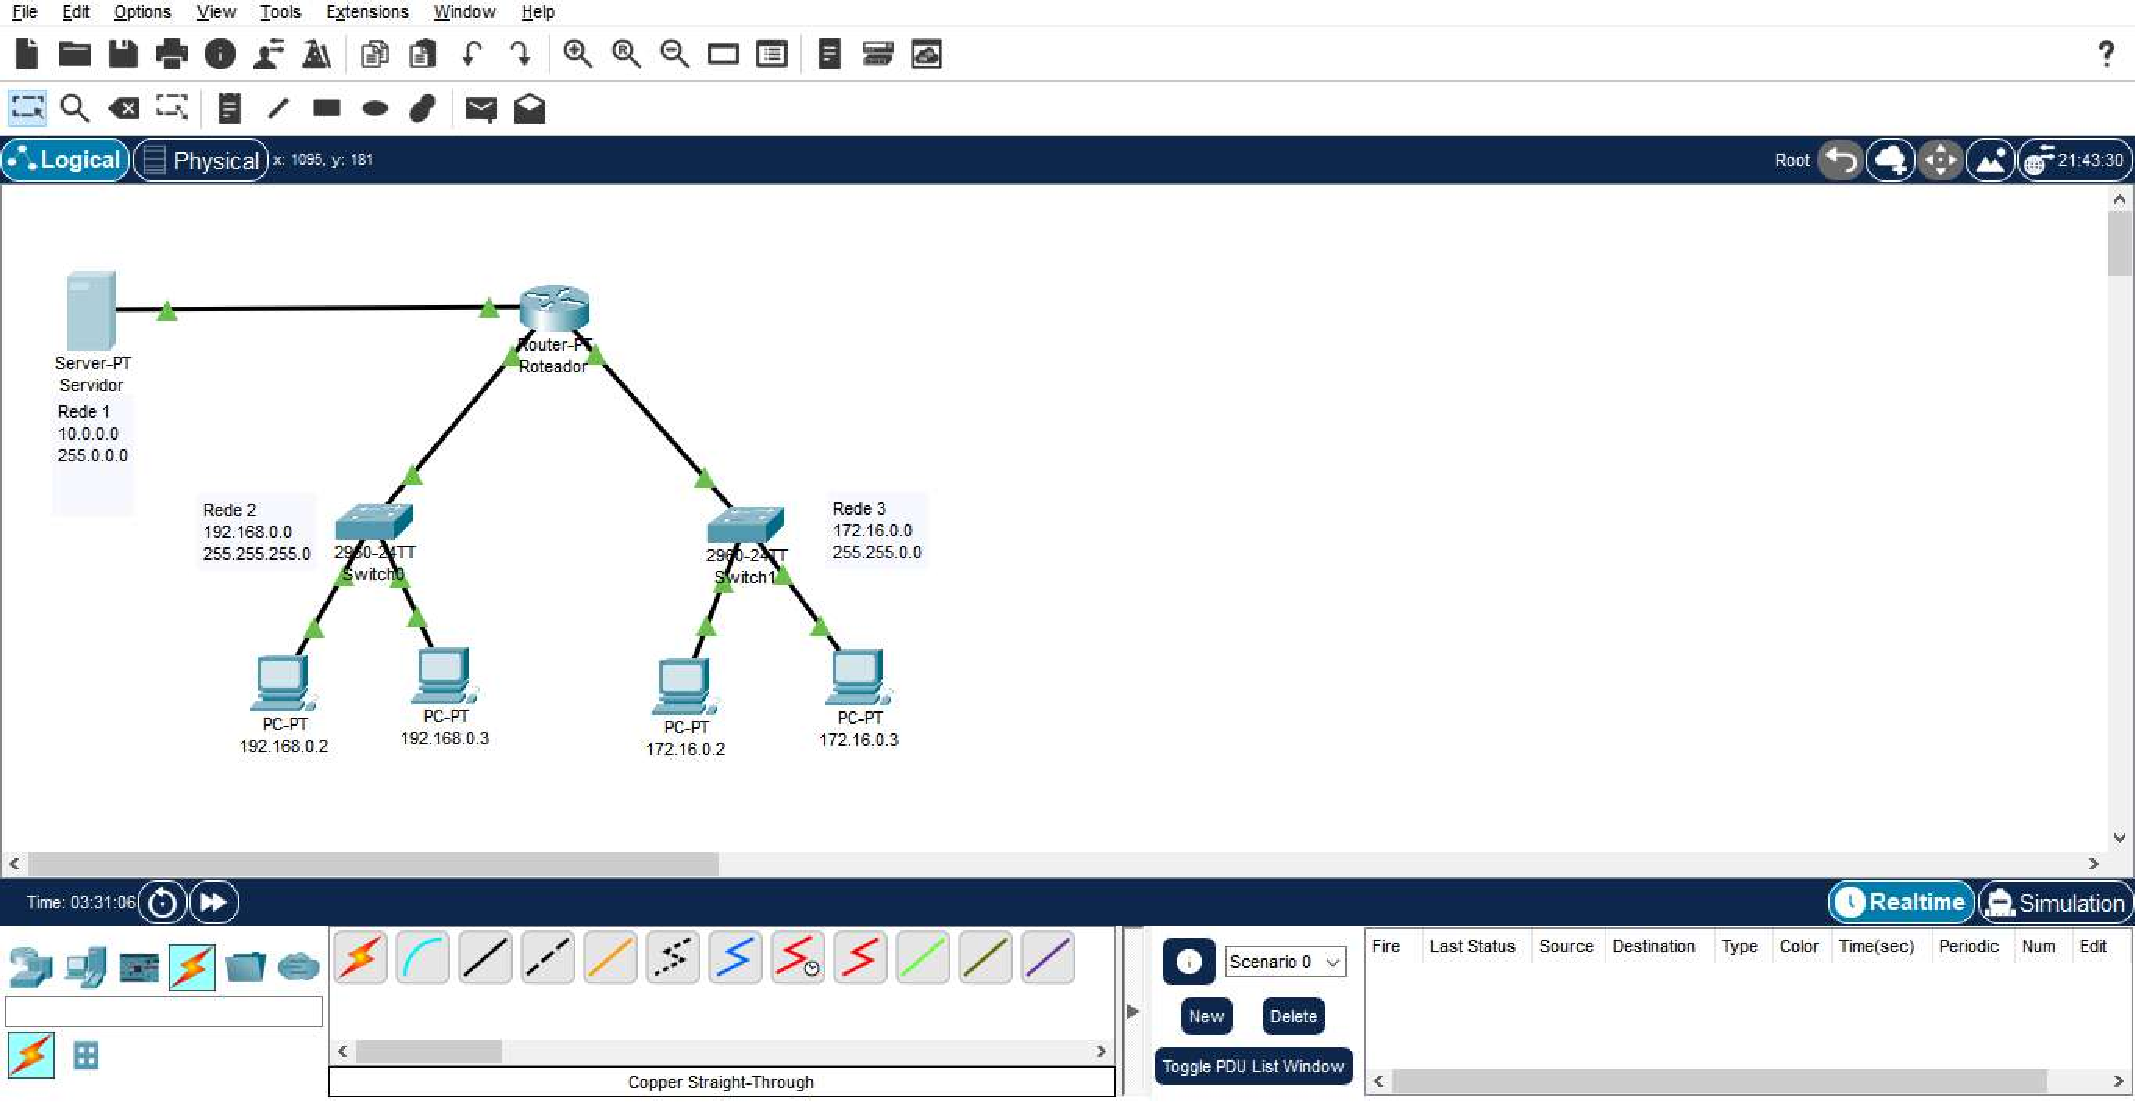
\includegraphics[width=.93\textwidth]{Figuras/firewallBase}
    \caption{Infraestrutura exemplo para a inclusão de \textit{firewall}.}\label{fig:firewallBase}
\end{figure}

\section{Configuração inicial do laboratório}\label{sec:configInicial}
Vamos detalhar as configurações atuais das redes. O servidor estará em uma rede local (LAN) composta apenas por ele mesmo. Note que o servidor possui com duas interfaces de rede, uma \textit{Gigabit Ethernet} e outra \textit{Fast Ethernet}. Nós utilizaremos apenas a \textit{Gigabit Ethernet}. O servidor terá o endereço IP \texttt{10.0.0.2} e estará na LAN \texttt{10.0.0.0}, com máscara \texttt{255.0.0.0}.  Chamaremos essa rede de \texttt{Rede 1} e o \textit{gateway} para essa rede será o \texttt{10.0.0.1}.

A \texttt{Rede 2} é composta por um \textit{switch} e dois PCs, tem endereço de rede \texttt{192.168.0.0} e máscara \texttt{255.255.255.0}. O primeiro PC tem o endereço IP \texttt{192.168.0.2} e o segundo PC tem o endereço IP \texttt{192.168.0.3}. Em ambos os casos, o \textit{gateway} será o \texttt{192.168.0.1}

Por sua vez, a \texttt{Rede 3} é composta por um \textit{switch} e dois PCs, tem endereço de rede \texttt{172.16.0.0} e máscara \texttt{255.255.0.0}. O primeiro PC tem o endereço IP \texttt{172.16.0.2} e o segundo PC tem o endereço IP \texttt{172.16.0.3}. Em ambos os casos, o \textit{gateway} será o \texttt{172.16.0.1}

Por fim, o roteador tem três interfaces \textit{Gigabit Ethernet} para se conectar ao servidor e as outras LANs. As interfaces têm as seguintes configurações:

\begin{itemize}
    \item A \texttt{GigabitEthernet0/0} tem endereço IP \texttt{10.0.0.1} e máscara \texttt{255.0.0.0}. Essa interface será ligada ao servidor.
    \item A \texttt{GigabitEthernet1/0} tem endereço IP \texttt{192.168.0.1} e máscara \texttt{255.255.255.0}. Essa interface será ligada ao \textit{switch} na \texttt{Rede 2}.
    \item A \texttt{GigabitEthernet2/0} tem endereço IP \texttt{172.16.0.1} e máscara \texttt{255.255.0.0}. Essa interface será ligada ao \textit{switch} na \texttt{Rede 3}.
\end{itemize}

Ainda no roteador, o roteamento escolhido foi o RIP e foram adicionadas as três redes \texttt{10.0.0.0}, \texttt{192.168.0.0} e \texttt{172.16.0.0}.

\section{Exercício}
Dada a configuração de rede atual, verifique se você consegue o seguinte:
\begin{itemize}
    \item Enviar um PDU de um PC na \texttt{Rede 1} para a \texttt{Rede 2}.
    \item Enviar um PDU de um PC na \texttt{Rede 1} para o servidor.
    \item Enviar um PDU do servidor para um PC na \texttt{Rede 2}.
\end{itemize}

Se não conseguiu, espere um pouco e tente novamente. É preciso algum tempo para as rotas estabilizarem.

\section{Configuração do \textit{Domain Name Service}}
Embora não seja necessário para a utilização do \textit{firewall}, para tornar o exemplo mais completo, vamos configurar um Sistema de Nomes de Domínio (\textit{Domain Name System} -- DNS) no próprio servidor. Basicamente um DNS é um sistema hierárquico e distribuído de gestão de nomes para  serviços ou qualquer máquina conectada à Internet ou a uma rede local. Em suma, o servidor DNS vai resolver um nome, isto é, traduzindo aquele nome em um endereço IP.

Para definir o DNS no servidor, basta seguir esses passos:
\begin{enumerate}[label*=\arabic*.]
\item Clique sobre o servidor, em seguida clique na aba \textit{Services}.
\item Na lateral esquerda, clique sobre a \textit{string}  \texttt{DNS}.
\item Na caixa de texto \textit{Name}, informe o nome do domínio que você vai definir. Nesse exemplo, colocamos o nome \semaspas{www.servidorft.com.br}.
\item Na caixa de texto \textit{Address}, defina o endereço IP daquele domínio que você vai definir. Nesse exemplo, colocamos o endereço \semaspas{10.0.0.2}. Note que é o endereço do próprio servidor, que também funcionará como servidor \textit{web}.
\item Depois de preenchidos o \textit{Name} e o \textit{Address}, clique no botão \keys{Add}.
\item Certifique-se que a configuração está salva, clicando no botão \keys{Save} e que o DNS está ativo selecionado a opção \textit{On} na parte superior.
\end{enumerate}

Agora, indique, em todos os PCs, o endereço do DNS está definido. Para isso, faça o seguinte em cada PC:

\begin{enumerate}[label*=\arabic*.]
\item Clique sobre o PC.
\item Selecione a aba \textit{Config}.
\item Informe o endereço IP \semaspas{10.0.0.2} na caixa de texto \textit{DNS Server}.
\end{enumerate}

\section{Exercício}
Escolha um PC na sua rede e verifique se o servidor \textit{Web} está ativo. Para isso, faça o seguinte:

\begin{enumerate}[label*=\arabic*.]
\item Clique sobre o PC.
\item Selecione a aba \textit{Desktop} e em seguida selecione o \textit{Web Browser}.
\item Na caixa de texto \textit{URL}, informe o nome do servidor \semaspas{www.servidorft.com.br}.
\end{enumerate}

Se deu certo, deve aparecer uma página com o título \textit{Cisco Packet Tracer}. Repita esse procedimento em todos os PCs, para se certificar que funciona para todos.

\section{Funcionamento básico do \textit{firewall}}\label{sec:funcBasicoFirewall}

Cada serviço disponível na rede está vinculado a uma porta específica. Por exemplo, o serviço \textit{web} que usa o  Protocolo de Transferência de Hipertexto (\textit{Hypertext Transfer Protocol} -- HTTP) usa a porta 80; o serviço FTP, usa a porta 21; e o serviço DNS usa a porta 53. Esses serviços também utilizam protocolos específicos na camada de transporte. Esses protocolos podem ser o Protocolo de Controle de Transmissão (\textit{Transmission Control Protocol} -- TCP) ou o Protocolo de Datagrama do Usuário (\textit{User Datagram Protocol} -- UDP).

Um \textit{firewall} permite ou nega acessos observando os protocolos utilizados, os endereços IP de origem e destino das conexões, e também as portas de origem e destino dos pacotes. Assim, as regras de segurança são estabelecidas com base nesses parâmetros.

\section{Configuração do \textit{firewall}}\label{sec:configFirewall}
Agora, faremos a configuração do \textit{firewall} no servidor. Para esse exemplo, vamos permitir (\textit{Allow}) o acesso dos PCs aos serviços DNS e \textit{Web}. Mais a frente, no exercício, terminaremos a configuração para negar (\textit{Deny}) o acesso dos PCs aos serviços ICMP e de transferência de arquivos (com o \textit{file transfer protocol} -- FTP). Lembrando que a negação do serviço ICMP vai evitar a conexão pelo comando \Comando{ping}.

Para configurar o \textit{firewall}, vamos executar os seguintes passos:

\begin{enumerate}[label*=\arabic*.]
\item Clique sobre o servidor e em seguida, clique na aba \textit{Desktop}.
\item Clique sobre o ícone do \textit{firewall IPv4}. Cuidado, pois também há o \textit{firewall IPv6} que não utilizaremos neste exemplo.
\item Na seção \textit{Service}, selecione a opção \textit{On} para deixar esse serviço ativo.
\item Na seção \textit{Interface}, selecione a opção \textit{GigabitEthernet1}, que é a interface a qual o \textit{firewall} vai observar.
\item Para permitir o serviço DNS faça o seguinte:  
   \begin{enumerate}[label*=\arabic*.]
      \item Na caixa de opções \textit{Action}, selecione \textit{Allow}.
      \item Na caixa de opções \textit{Protocol}, selecione \textit{UDP}.
      \item Na caixa de texto \textit{Remote IP}, preencha com o endereço IP da rede da qual virão os pacotes (nesse exemplo, a rede \texttt{192.168.0.0}).
      \item Na caixa de texto \textit{Remote Wildcard Mask}, preencha com a máscara invertida da rede da qual virão os pacotes (nesse exemplo, a máscara da rede é \texttt{255.255.255.0} e a máscara invertida -- que você deverá preencher -- é a \texttt{0.0.0.255}).
      \item Na caixa de texto \textit{Remote port}, preencha com a \textit{string} \texttt{any}. Essa \textit{string} informa que a porta de origem da conexão pode ser qualquer uma.
      \item Na caixa de texto \textit{Local port}, informe a porta 53 (a porta do serviço DNS).
      \item Depois que as informações forem preenchidas, clique em \keys{Add}.
   \end{enumerate}
\item Para permitir o serviço \textit{Web} repita o procedimento do item 5, substituindo o seguinte:
   \begin{enumerate}[label*=\arabic*.]
      \item Substituir o protocolo (no item 5.2) por \textit{TCP}.
      \item Substituir a \textit{Local port} (no item 5.6), pela porta 80 (a porta do serviço \textit{web}).
    \end{enumerate}
\end{enumerate}

A negação dos serviços ocorre de forma similar à liberação. A diferença é que, na caixa de opções \textit{Action}, você deve selecionar a opção \textit{Deny}. 

\section{Exercício}
Na \Cref{sec:configFirewall}, fizemos a configuração do \textit{firewall} para permitir dois serviços (DNS e \textit{web}) para a \texttt{Rede 2} (\texttt{192.168.0.0}). Nesse exercício, termine a configuração para bloquear o protocolo ICMP e o FTP na Rede 2 e faça a configuração completa para a \texttt{Rede 3} (\texttt{172.16.0.0}). Lembrando que o serviço FTP utiliza o protocolo TCP na camada de transporte e atua na porta 21. O serviço ICMP também utiliza o protocolo TCP na camada de transporte e atua na porta 23.

Ao final, a configuração do \textit{firewall} deve ficar conforme a \Cref{fig:configFirewall}. Depois que a configuração do \textit{firewall} estiver completa, faça testes para verificar se os serviços estão realmente bloqueados e liberados. 

\begin{figure}[!htb]
    \centering
    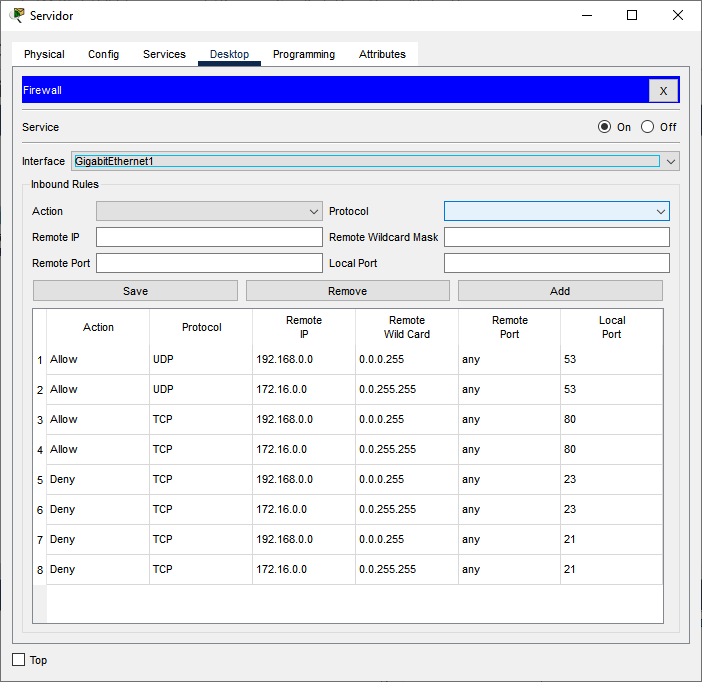
\includegraphics[width=.9\textwidth]{Figuras/configFirewall}
    \caption{Configuração final do \textit{firewall} no exemplo.}\label{fig:configFirewall}
\end{figure}